\section{Security considerations}
In order to increase the level of security in our system, different considerations should be made. These considerations are made in order to make it more difficult for intruders to break into the system as well as hide personal sensitive information. We limit the discussion to program communication and how we handle personal sensitive information, as this is where we assess the system have the biggest weaknesses.
\ofx{tie this to sprint1 security} \sfx{Is it necessary to emphasize that we aren't security experts?}

\subsection*{HTTPS} 
%  HTTPS and SSL certificate. May want to talk more about where we could use it in our system
The system currently uses HTTP, an insecure communication protocol that uses cleartext to communicate. Anybody intercepting the communication can read it with ease. We can diminish the damage from this attack by using the HTTPS protocol, short for \textit{Hyper Text Transfer Protocol Secure}, which functions as the HTTP protocol with the exception that the message is encrypted. This means that if someone were to gain access to the connection they would not be able to read the information. A secure connection is very important on sites that handle sensitive information such as CPR-numbers or credit card information and this can be achieved by using HTTPS\cite{HTTPS}.

\begin{figure}[ht]
	\begin{center}
		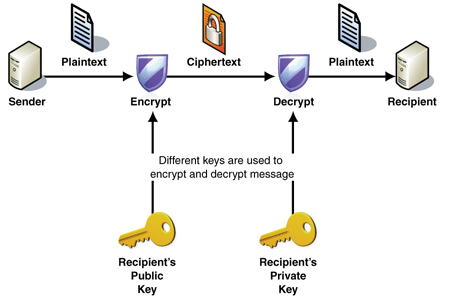
\includegraphics[scale=0.9]{graphics/HTTPS.png}
		\caption{HTTPS \cite{https_pic}.}
		\label{fig:HTTPS}
	\end{center} 
\end{figure}

\Cref{fig:HTTPS} shows how HTTPS works after the key exchange have taken place. First the sender sends plain text, which is encrypted using the recipients public key. The encrypted message is then sent and decrypted using the recipients private key before plain text is received.

The handshake between the browser and a site using HTTPS starts with an exchange of public SSL-keys (Secure Socket Layer). The SSL-key is unique and enables encryption of the data sent. The encrypted data can then only be decrypted with your own private key\cite{HTTPS}. \sfx{I'm not sure it's necessary to explain how HTTPS works in this amount of detail. If it is, we need to rewrite it. It is not very clear here.}

\subsection*{Certificates}
Initially we created an empty certificate-handler which is still in use. This means that the certificates are accepted no matter what, which is very insecure. An alternative, more secure solution, would be to download the certificates and insert them in the JVM keystore, which is a collection of all accepted certificates. By freely accepting all certificates it is possible for attackers to input dirty data in the system by adding a server pretending to be an MSE service.

\subsection*{Hashing}
Hash functions are most commonly used to store a users password or other sensitive data. It functions as a one way mapping; when a message is hashed it can not be reversed again. The formal definition is shown below:
\begin{quote}
\textit{'A hash function is a computationally efficient function mapping binary strings of arbitrary length to binary strings of some fixed length, called hash-values.'\cite{Hash_def}}
\end{quote}

It has been requested by the Heatmap application group to have a unique identification of all people. If we are not allowed to store the MAC-Address, a solution to this would be to hash the MAC-Address with a random, changing salt. In this way it will be possible for the application to track people for as long as the salt-value is unchanged.

Java has a hash-method implemented in the object class called \textit{hashCode()}, this may be used for hashing information. When using a hash function, you add a randomly generated string that extends the original message. The generated string is called a salt and makes the hash function more secure.

\subsection*{Hard-coded passwords}
When communicating with MSE from the intermediate server as well as when communicating with the intermediate server, we are currently using hard-coded passwords. This means that everyone with access to the code can find the log-in information. The information should be given as arguments to the program and hashed such that the log-in can not be seen in the code and cannot be read as plain text in memory. 

\subsection*{Visibility}
As of now many parts of the system has a higher degree of visibility than necessary. This makes it possible to use functionality in unexpected ways and possibly cause unintended behaviour. We can decrease the level of visibility by having private and protected classes and methods, which leads to a system that is more resilient towards unexpected usage.
 
\subsection*{Obfuscate personal information}
In order to ensure our users personal information, we decided to obfuscate the E-mail addresses in the same manner as it is done to the MAC-address. By doing so there will be no way for outsiders to identify people unwilling to have their information stored.

\subsubsection*{IP-address}
IP addresses are not considered personal information. This is based on the fact that IP changes each time you change access point. By not obfuscating the IP it open up possibilities to the apps, they will be able to see how many people are connected to a given access point. 